\documentclass[conference]{IEEEtran}
\IEEEoverridecommandlockouts
% The preceding line is only needed to identify funding in the first footnote. If that is unneeded, please comment it out.
\usepackage{amsmath,amssymb,amsfonts}
\usepackage{algorithmic}
\usepackage{graphicx}
\usepackage{textcomp}
\usepackage{xcolor}
\usepackage{biblatex}
\addbibresource{bibfile.bib}

\def\BibTeX{{\rm B\kern-.05em{\sc i\kern-.025em b}\kern-.08em
    T\kern-.1667em\lower.7ex\hbox{E}\kern-.125emX}}
\begin{document}

\title{Real Time 3D Sound Hardware Implementation\\
}

\author{
\centering
\IEEEauthorblockN{Sathwik GS, Barun Kumar Acharya, Bilal Ali}
\IEEEauthorblockA{Department of Electronics and Communication Engineering \\
National Institute of Techonology Karnataka, Surathkal, India\\
Email: sathwikgs97@gmail.com}
}

\maketitle

\begin{abstract}
3D Audio is a generic name that allows to render and recreate audio as experienced in reality, with spatial dimension being the main parameter. To synthesize the 3D sound effects with a binaural recording system, Head-related transfer functions (HRTFs) were used describing the spectral behaviour of sounds coming from a particular direction. In this paper we implement a hardware design to realise the effect of 3D sound by efficient processing of time varying FIR filters and verify its functionality in real time using a FPGA.  

\end{abstract}

\begin{IEEEkeywords}
Binaural recording, HRTFs, 3D audio, Real time hardware design
\end{IEEEkeywords}

\section{Introduction}
For many years now Binaural recording has been the most commonly used method to provide an immersive sound experience. The method involves using artificial or dummy heads plugged in with microphones to record and reproduce the same over headphones. But this type recording requires special equipment and is not as portable as any other two channel recording instrument. 
HRTFs (Head related Transfer Function) describe how a sound from a specific point will arrive at the ear (generally at the outer end of the auditory canal). These impulse responses are typically recorded in an anechoic chamber to minimize the influence of early reflections and reverberation on the measured response. They are measured at small increments of θ such as 15$^{\circ}$ or 30$^{\circ}$ in the horizontal plane. The brain has learned these signature over time and when it hears a sound with a specific signature, it can find out the direction in its HRTF memory. A pair of HRTFs for two ears can be used to synthesize a binaural sound that seems to come from a particular point in space. In this paper we design an ASIC to synthesize sounds using HRTFs and also test it by implementing on a FPGA.  
\newline

Initially researchers were interested in localizing the sound source rather than reproducing it. Several methods have been proposed in different transfer domains to increase the computational speed of localizing. One of the most robust methods is the GCC (Generalised Cross Correlation) technique as discussed by Knapp and Carter \cite{two} where along with basic cross-correlation, a weighting function is applied to the power spectrum. Among different weighing functions, the most popular one called GCC-PHAT was introduced by Broeck and Bertrand \cite{one}. This weighing scheme was used to achieve unity gain on all frequency components with preservation of phases.  This was designed for locating only single sound source. However it was modified for more critical situations such as multiple sources, described in \cite{three}. The technology of surround sound systems was invented back in 1930s. During the early stages, audio engineers used a procedure called amplitude panning, which allows audio sources like instruments to be placed in different positions to build up a sound scene utilising the panning law, or sometimes to place the source around a listener in the horizontal plane. The technique lacked reproduction of frequency information for different spatial positions. It was then important to understand the working of human ears particularly in the frequency domain. The basic concepts of 3D sound systems are explained in detail by Wenzel \cite{four}. Alongside development in recording technology and signal processing techniques, 3D reproduction of sound was then realized on the basis of HRTFs from source to the right and left ears as discussed by Chong-Jin and Gan \cite{six} and Wenzel \cite{four}. The  robustness  analysis,  localization  characteristics,  structural  model  for  binaural  sound  synthesis  and  head related transfer functions are discussed in detail by Brown and Duda \cite{seven}. All these methods help in reproduction of 3D sound using HRTFs, but not in real-time. There is no emphasis on efficient computation to achieve the same.  

In this paper we discuss the hardware implementation to realise 3D sound effect in real time. We also address methods to efficiently execute time varying FIR filters. This paper is organized into four sections. Section II explains the algorithm which is required to be implemented. Section III describes the implementation details and Section IV analyzes the results obtained from tests and experiments conducted.  


\section{Algorithm}

Since convolution of the audio signals with HRTF corresponding to a particular direction makes it seem as if the sound source is placed in that spatial area, it is important to first locate the source. The designed system records samples using microphones separated 20cm apart (approximate distance between the ears) at a standard rate of 44.1 kHz. Filters from one of the most popular databases - CIPIC HRTF database \cite{cipic}, are used to convolve any incoming audio signal. The original filter length of 200 coefficients were downsampled in frequency domain and converted to a 100 tap filter to reduce the number of computations but not reduced further to preserve the frequency resolution.

The received audio signals on both the channels \textit{l(t)} and \textit{r(t)} are cross-correlated to estimate the delay or the time difference of arrival of signals. The angle of sound source is then estimated as follows: 

\begin{equation}
\tau = \frac{Max(\textit{l(t)} * \textit{r(t)}) - Signal length}{44100} 
\label{tdelay}
\end{equation}
where $\tau$ is the delay between the two signals (in seconds) and '*' is the cross-correlation operation whose index of maximum value is returned. Length of signals correlated is 100 samples long. 

\begin{equation}
sin\theta = \frac{\tau c}{d}
\label{angle}
\end{equation}
where c is speed of sound = 343 m/s , d is 20cm, $\theta$ is the azimuthal angle estimated.

Given that the database has 25 different azimuths, using $\theta$ derived, a filter corresponding to the closest angle is chosen.         

\section{RTL Design}
The top level design looks as shown in Fig \ref{fig:top_level}

\begin{figure}
    \centering
    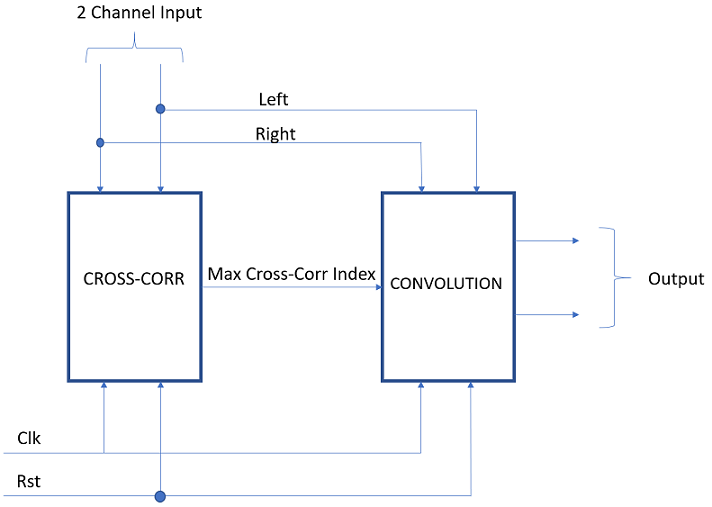
\includegraphics[width = 8cm, height = 4.5cm]{overall_design.png}
    \caption{Top Level}
    \label{fig:top_level}
\end{figure}

\subsection{Data Format}
The RTL design assumes data to be in the following format: 
\begin{itemize}
    \item Inputs/Outputs: Signed 16 bits 
    \item Each value in Q1.15 format where MSB bit is the sign bit and remaining 15 bits are the fractional bits
    \item Range of values should be from -1 to 1 
\end{itemize}

\subsection{MAC Unit}
This is the only arithmetic unit of the design. It uses one multiplier and adder, as shown in Fig \ref{fig:mac}. The result is stored in a 16 bit register. 

\begin{figure}
    \centering
    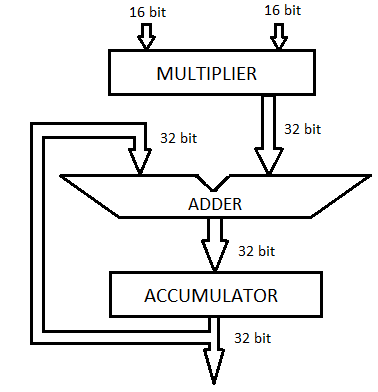
\includegraphics[height = 4cm]{mac.png}
    \caption{MAC Unit}
    \label{fig:mac}
\end{figure}
\subsection{Cross-Correlation Module}
This unit cross-correlates data buffers 100 samples long and returns the index of maximum value. One of the buffers is extended to a length of 298 samples but non-zero samples present only in indexes 100 to 199, rest filled with zeros. This is done so that only the smaller buffer is slid over the other corresponding to each shift. The correlation is done by performing MAC operation on each shift, illustrated in Fig \ref{fig:xcorrflow}  and The whole operation is divided into two parts: Data acquisition and Correlation computation. The samples are collected at every 5th data frame and the computation is done over the period of 4 data frames, Fig \ref{fig:modxcorr}. 

\begin{figure}
    \centering
    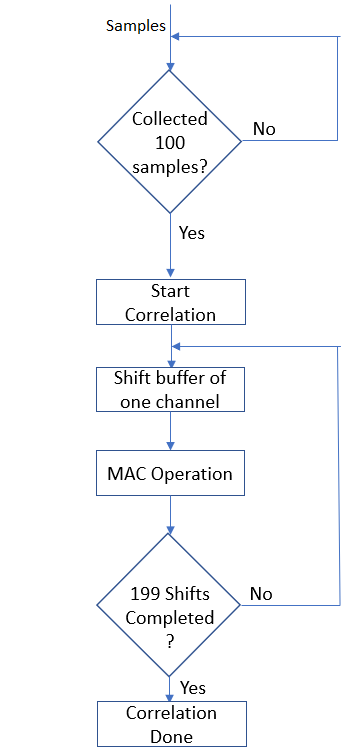
\includegraphics[height = 8cm]{xcorr_flow.png}
    \caption{Data Flow}
    \label{fig:xcorrflow}
\end{figure}

\begin{figure}
    \centering
    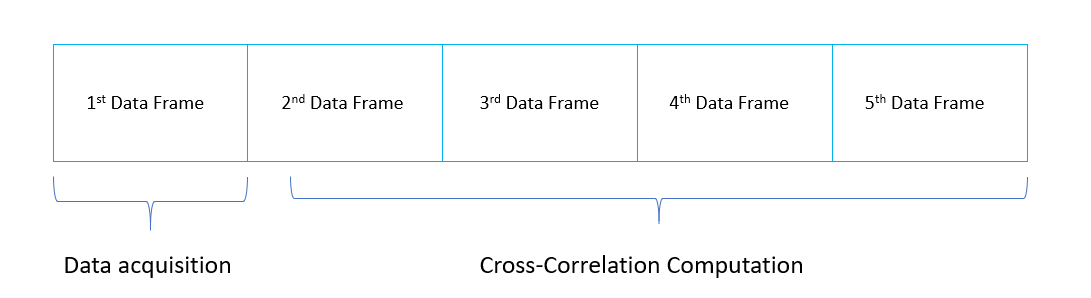
\includegraphics[height = 3cm, width = 7cm]{modified_xcorr.png}
    \caption{Pipeline for cross-correlation}
    \label{fig:modxcorr}
\end{figure}

Each shift in the computation requires 100 MAC operations, hence with 199 shifts we require 19900 operations to be completed in the time period of 4 data frames = 400 sample periods. Clock speed required for MAC is at least 50 times faster than sampling rate. This corresponds to having 50 MAC operations per sample period with 100 clock periods as idle time in the end.

\subsection{Convolution Module}
Every data frame of 100 samples is convolved with a filter chosen according to the index given by the correlation module. Each output sample is computed by 100 MAC operations, Fig \ref{fig:conv_module}. Even though the correlation module requires only 50 times faster clock speed, but this module requires 100 times faster = 4.41 MHz. 

\begin{figure}
    \centering
    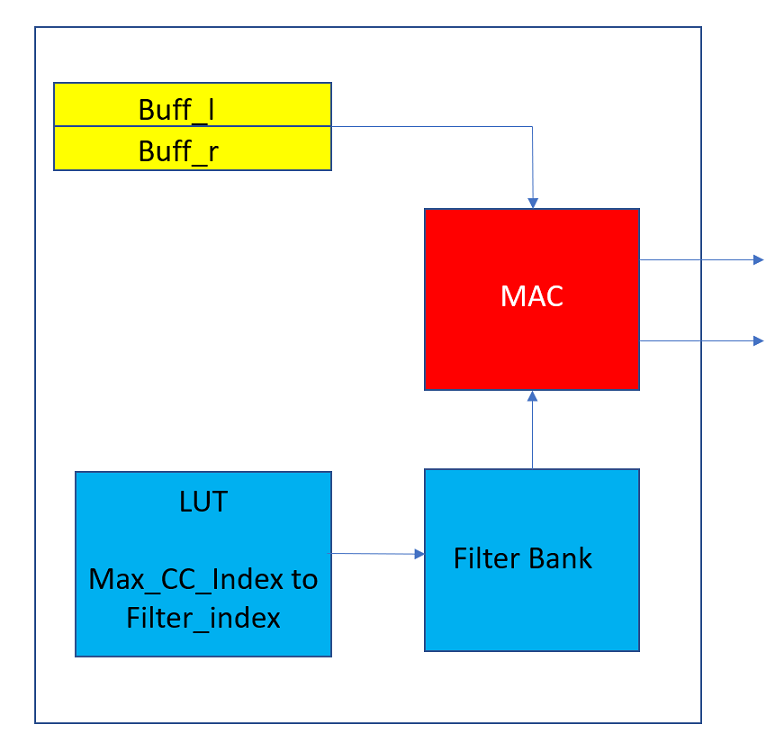
\includegraphics[width = 5cm, height = 4cm]{conv_module.png}
    \caption{Convolution Module}
    \label{fig:conv_module}
\end{figure}

Not every result of cross-correlated index mapped to a filter is chosen and convolved, instead past 10 outputs are stored and the filter mapped the most number of times is finally chosen, Fig \ref{fig:past10}. This means that there is a possibility of a filter change at every 50$^{th}$ data frame , i.e. at about 110 ms which can account for any change in the position of sound source.

\begin{figure}
    \centering
    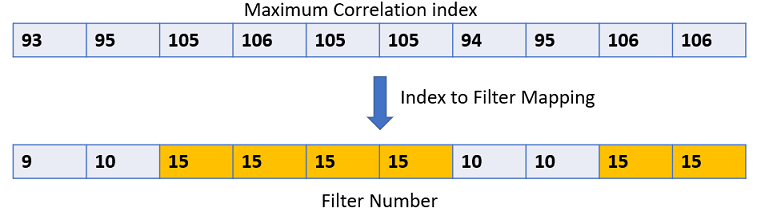
\includegraphics[width = 8cm, height = 2.5cm]{index_2_filter.png}
    \caption{Example of Filter Selection}
    \label{fig:past10}
\end{figure}

\subsection{Convolution during filter change}

For 50 frames of data, a fixed filter is used after which there can be a change in filter. Changing the entire filter buffer with the new set of coefficients would be incorrect since convolution with the previous filter would be incomplete. Two convolution units are required at the same time, One - to finish the ongoing convolution process and second - to begin filtering with the new one.

However, this requirement can be avoided by carefully observing the impact of coefficients on the output. We use the \textit{stepwise replacement of impulse response} method as mentioned in \cite{live} but in time domain to achieve the same result, Fig \ref{fig:coeffupdate}. The coefficients are updated in the filter buffer at the same sampling rate. Primary advantage being that only 1 convolution unit is being used all the time. A register is required to keep storing the previous filter chosen. 

\begin{figure}
    \centering
    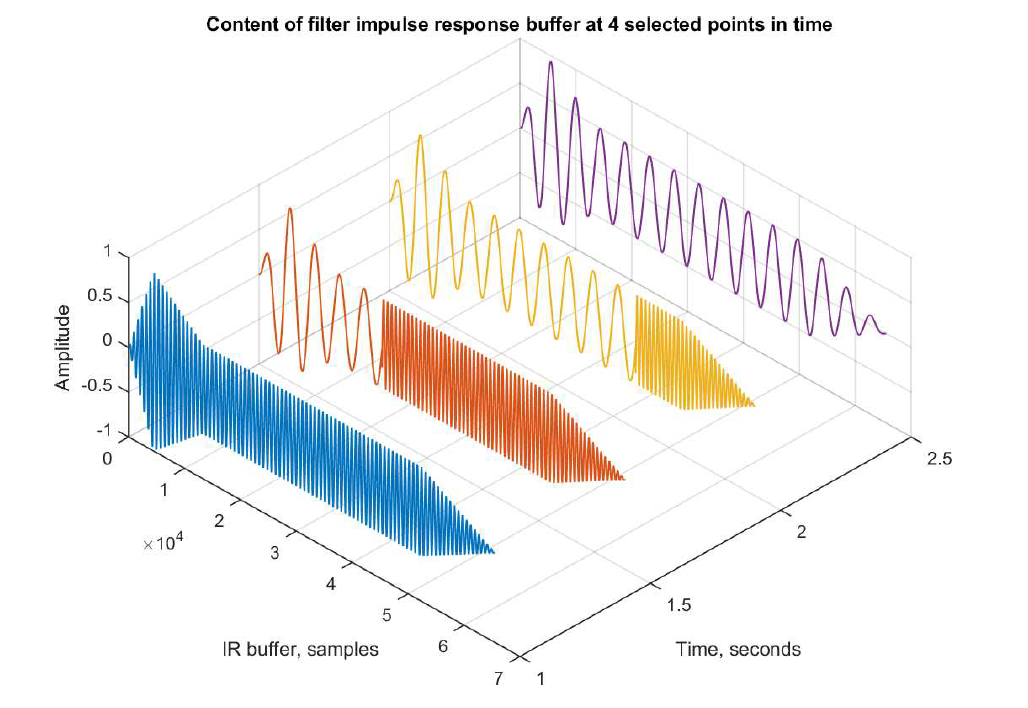
\includegraphics[width = 8cm]{coeffupdate.png}
    \caption{Partial Coefficient Buffer, \cite{live}}
    \label{fig:coeffupdate}
\end{figure}

\subsection{Smooth transition}
 To avoid audible glitches during transition, along with the method of convolution explained above it is important to crossfade between the two outputs. This is illustrated in Fig \ref{fig:crossfade}. 
 For $0<n<n_l$
 \begin{equation}
     filter \textunderscore buffer(n) = H(prev)*fade \textunderscore out + H(curr)*fade \textunderscore in
 \end{equation}
 for $n_l<n<100$ 
 \begin{equation}
     filter \textunderscore buffer(n) =  H(prev)
 \end{equation}
 where $0<n_l<100$ increments at sampling rate and \textit{H} contains filter coefficients.
 \begin{figure}
     \centering
     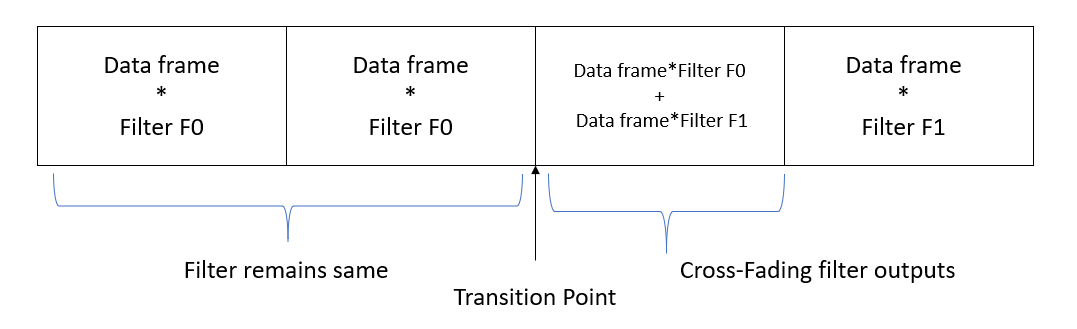
\includegraphics[width = 10cm]{Crossfade.png}
     \caption{Transition between filters}
     \label{fig:crossfade}
 \end{figure}
 
 Standard fading techniques such as linear, square-root, sin-cos can be used. But it is easier to implement linear fadein/out as no memory is required to store them. They can be dynamically generated , Fig \ref{fig:fadegen}. The inital values for fade\textunderscore out and  fade\textunderscore are 0x7FFF and 0x0000 respectively . To completely fade in/out within 100 samples the difference between their adjacent values = 0x014B. 
 \begin{figure}
     \centering
     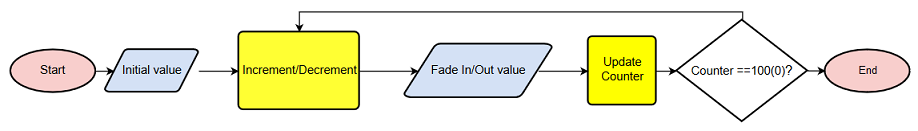
\includegraphics[width = \linewidth, height = 2cm]{fade_gen.png}
     \caption{Fade In/Out Generator}
     \label{fig:fadegen}
 \end{figure}
 
\section{Implementation Results}

Synthesis of design was done using SCL 0.18 $\mu$m libraries. To verify the functionality of detecting angle of sound source, recorded samples were given as input in the post synthesis simulation of the design. Samples were recorded with National Instruments Data Acquisition device at a sampling rate of 44.1 kHz. The experiment involved placing the sound source at 40$^\circ$ to the right from center of the microphones. Fig \ref{fig:right} clearly indicates that the source was placed at an angle corresponding to index 116. Using equation \ref{tdelay} and \ref{angle} this index maps to angle = 38.47$^\circ$ Although the module resulted in other indexes but having a scheme as shown in Fig \ref{fig:past10} helps in minimal acceptance of them. Another experiment involved moving the source continuously from left to center (and vice versa). Fig \ref{fig:left} shows the resulting indexes. The resultant mapping ranges from 30$^\circ$ to the left to center. Apart from central position most of the angles occur equally likely, indicating constant movement. 

\begin{figure}
    \centering
    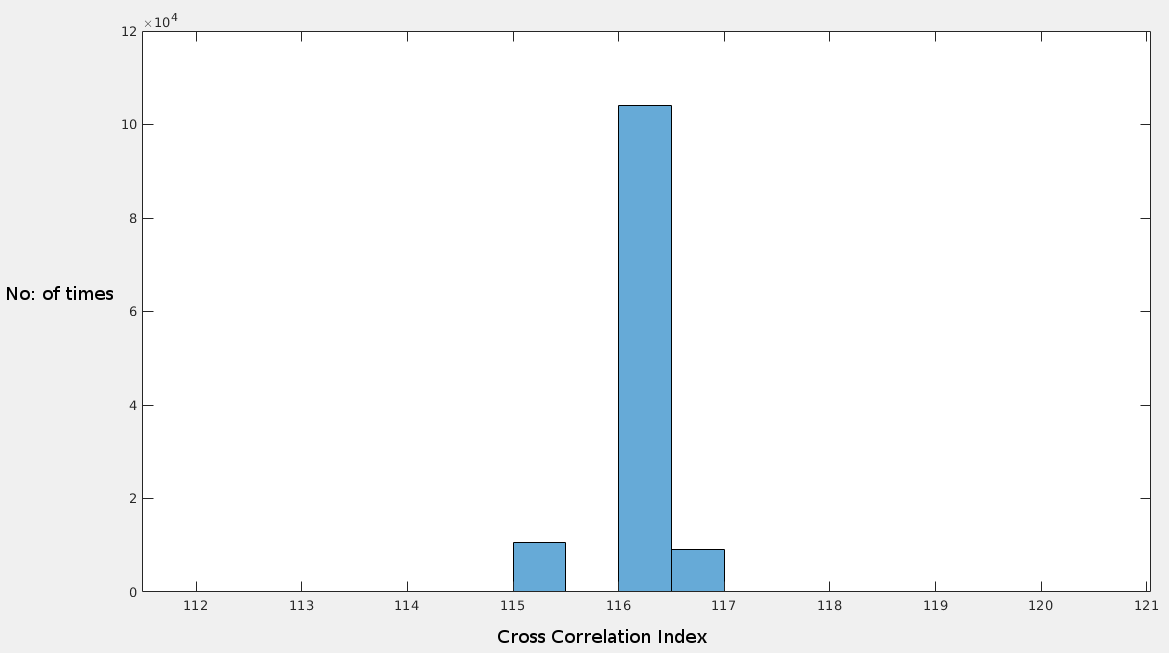
\includegraphics[width = 9cm]{right.png}
    \caption{True angle of source = 40$^\circ$}
    \label{fig:right}
\end{figure}

\begin{figure}
    \centering
    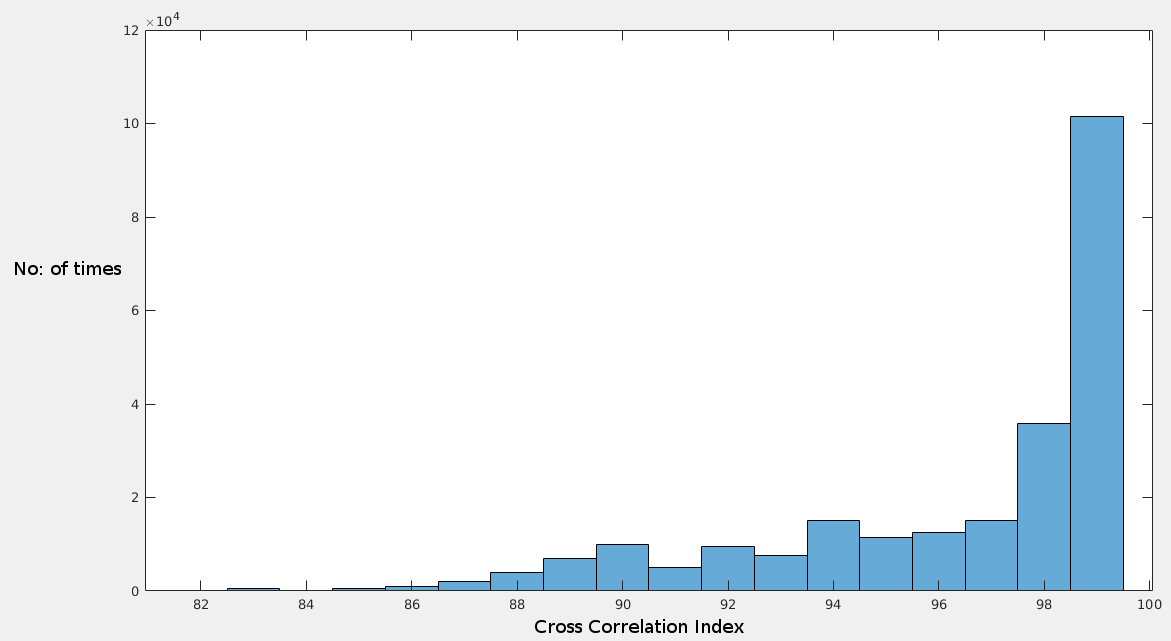
\includegraphics[width = 9cm]{left.png}
    \caption{Continuous movement of source ranging from left to center}
    \label{fig:left}
\end{figure}

In order to test the design and check its functionality in real time Xilinx Nexys 4 DDR Artix -7 FPGA was used. Initally, experiments were conducted to realise the effect of HRTFs by manually changing the filters. This is also known as panning where the end effect is as if the sound source is moving around user's head. ADMP401 MEMS microphones which are omnidirectional, low power and has a flat frequency response from 100Hz to 15kHz was used as input (analog). Nexys 4 has \textit{XADC}, which is a 12-bit dual channel ADC with 1 MSPS (Mega Samples per Second) which converts the microphone output to a 16-bit digital signal. The output is converted back to its analog equivalent using \textit{PMOD I2S DAC} module which uses the I2S protocol. The resultant output was as expected, i.e. periodic change in filter resulted in panning effect.

After functional verification of HRTFs, the proposed design was implemented to automatically detect the angle of source and accordingly choose the filter, Fig \ref{fig:setup}.
The resource utilization is given in Table \ref{tab:resourceuti}. Here all the filter coefficients were directly stored in registers, taking up most of the resources. Had there been external memory interfacing the utilized resources would come down.  As expected, the RTL design implemented was able to locate the sound source. The movement of source was accurately tracked and helped in filter selection. Subjecting to listening test, the user was able to realise the 3D sound effect. \newline


\begin{figure}
    \centering
    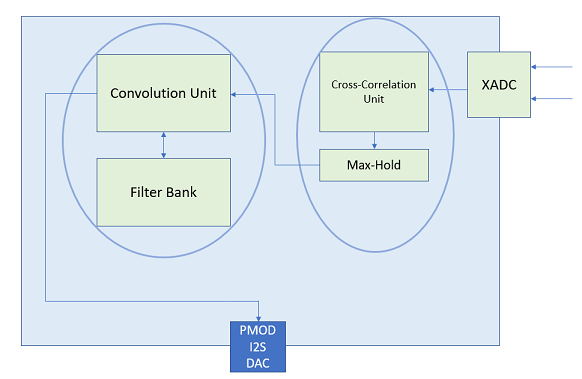
\includegraphics[width = 8cm, height = 5cm]{fpga_layout.png}
    \caption{Block Representation}
    \label{fig:setup}
\end{figure}
\begin{table}[]
    \centering
    \begin{tabular}{ |c|c|c|c| } 
         \hline
         \textbf{Resource} & \textbf{Utilization} & \textbf{Available} & \textbf{Utilization} \% \\ 
         \hline
         LUT & 7957 & 63400 & 12.55\\ 
         FF & 1678 & 126800 & 1.32\\
         DSP & 2 & 240 & 0.83 \\
         IO & 36 & 210 & 17.14 \\
         BUFG & 8 & 32 & 25.00 \\
         MMCM & 1 & 6 & 16.67\\
         \hline
    \end{tabular}

    \caption{Resource Utilization}
    \label{tab:resourceuti}
\end{table}

\section{Conclusion}

A real-time implementation of the proposed design was done and its various characteristics was discussed in this paper. Functional verification was done through post synthesis simulation and real time testing was conducted on FPGA. The design and algorithm worked as expected enabling the user to realise 3D sound via headphones.

\printbibliography

\end{document}
